\section{Introduction}
\label{sec:intro}
\label{sec:intro:context}

In the specification of a concurrent programming language or a
parallel architecture, the \emph{memory consistency model} (MCM)
defines which values can legally be read from shared memory
locations~\cite{adve+96}. MCMs have to be general enough to enable
portability, but specific enough to enable efficient
implementations. They must also admit optimisations employed by architectures (such as
store buffering and instruction reordering~\cite{hennessy+12}) and by
compilers (such as common subexpression elimination and constant
propagation~\cite{aho+06}). This profusion of design goals has led to MCMs for
languages (such as C11~\cite{c11} and OpenCL~2.0~\cite{opencl20}), for
CPU architectures (such as x86, ARM, and IBM Power), and for GPU
architectures (such as AMD and NVIDIA), that are complicated and
counterintuitive. In particular, all of these MCMs permit executions
that are not \emph{sequentially consistent} (SC), which means that
they do not correspond to a simple interleaving of concurrent
instructions~\cite{lamport79}. As a result, designing and reasoning
about MCMs is extremely challenging.

Responding to this challenge, researchers have built numerous
automatic tools (see~\S\ref{sec:related}). These typically address the
question of whether a program $P$, executed under an MCM $M$, can
reach the final state $\sigma$. Put another way: can the \emph{litmus
test} $(P,\sigma)$ \emph{pass} under $M$? While useful, there are
several other questions whose answers are valuable for MCM reasoning
and development. Four that have appeared frequently in the literature
are:

\begin{description}
%
\item[\Q1] Which programs can be run to test whether a
compiler or machine conforms to a given MCM?~\cite{darbari+16,
alglave+10}
%
\item[\Q2] Is one MCM more permissive than another? That is, is there
a litmus test that can pass under one but must fail under the
other?~\cite{owens+09, mador-haim+12, mador-haim+10, batty+16,
nienhuis+16, lahav+16, alglave+10}
%
\item[\Q3] Can `strengthening' a program (syntactically) ever enable
additional behaviours?  For instance, can we take a litmus test that
must fail, impose additional sequencing or dependencies between its
instructions (or, in the C11 case, give an atomic operation a stronger
`memory order'~\cite[§7.17.3]{c11}), and thereby allow it to
pass?~\cite{sevcik+08, sevcik11, morisset+13, vafeiadis+15,
chakraborty+16, burckhardt+10}
%
\item[\Q4] Is a given software/architecture compiler mapping correct?
Or is there a litmus test that must fail under the software-level MCM,
but which, when compiled, can pass under the architecture-level
MCM?~\cite{batty+11, batty+12, wickerson+15a, sevcik+11, lustig+14, lustig+15}
%
\end{description}
%
% We note that each work cited above addresses one question in
% \emph{isolation} and, except for \Q1 and Lustig et al.'s
% work~\cite{lustig+14, lustig+15}, provides no automated methods for exploring
% the question.

\subsection{Key Idea 1: Generalising the Question}
\label{sec:intro:contribs}

Our first key idea is the observation that all four of the questions
listed above can be answered, sometimes positively and sometimes negatively, by exhibiting programs $P$ and $Q$ and state
$\sigma$ such that the litmus test $(P,\sigma)$ \emph{must fail} under
a given MCM $M$, $P$ and $Q$ are related by a given binary relation
$\blacktriangleright$ on programs, and $(Q,\sigma)$ \emph{can pass}
under a given MCM $N$. That is, each corresponds to finding inhabitants of
the following set.

\begin{definition}[General problem] 
\label{def:general_problem_programs}
%
$\GeneralProg(M,N,\blacktriangleright) \eqdef {}$
\[
\{(P,Q,\sigma) \mid \stack{\sigma \notin \obs_{M}(P) \wedge 
P\blacktriangleright Q \wedge \sigma \in \obs_{N}(Q)\}}
\] 
where $\obs$ returns the set of final states that can be observed
after executing a given program under a given MCM.\footnote{Elements of $\GeneralProg(M,N,\blacktriangleright)$
can also be seen as counterexamples to 
$\blacktriangleright$ implying observational
refinement~\cite{hoare72}:
$P\blacktriangleright Q \nRightarrow \obs_{N}(Q)\subseteq
\obs_{M}(P)$.}
\end{definition}


Our four questions correspond to the following specialisations of
$\GeneralProg$'s parameters:
%
\begin{description}
%
\item[\Q1] $\GeneralProg(M,\mm{0},\id)$ consists of tests that check conformance to $M$, where $\mm{0}$ is the MCM
that allows all executions and $\id$ is the identity relation;
%
\item[\Q2] $\GeneralProg(M,N,\id)$ consists of tests that cannot pass
under $M$ but can under $N$;
%
\item[\Q3] $\GeneralProg(M,M,\text{`is weaker than'})$ consists of
monotonicity violations in $M$, given a relation that holds when one
program is (syntactically) `weaker than' another; and
%
\item[\Q4] $\GeneralProg(M,N,\text{`compiles to'})$ consists of bugs
in a compiler mapping from $M$ to $N$, given a relation that holds when one program `compiles to' another.
%
\end{description}

\subsection{Key Idea 2: Constraining Executions, not Programs} 
\label{sec:intro:constraining_execs}

Having captured in Def.~\ref{def:general_problem_programs} our four
questions, we now ask whether answers can be generated using an
automatic constraint solver. Unfortunately,
Def.~\ref{def:general_problem_programs} is problematic because showing
that a litmus test must fail under $M$ requires universal
quantification over executions. That is, we must show that there
\emph{exists} a litmus test $(P,\sigma)$ such that \emph{all} possible
executions of $P$ under $M$ do not reach $\sigma$. As Milicevic et al.
observe, `this ``$\exists\forall$'' quantifier pattern is a
particularly difficult instance of higher-order
quantification'~\cite{milicevic+15}, and our pilot experiments
confirmed it to be intractable in practice.

\begin{figure}[t]
\centering
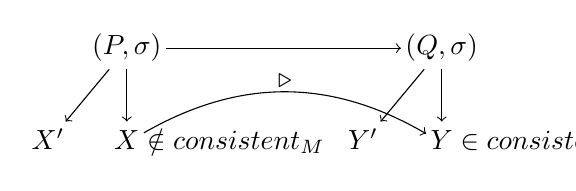
\begin{tikzpicture}[inner sep=0.5mm]
\node(P) at (1,1.2) {\strut $(P,\sigma)$};
\node(Q) at (5,1.2) {\strut $(Q,\sigma)$};
\node(X) at (1,0) {\strut \rlap{$X \notin consistent_M$}\phantom{$X$}};
\node(X') at (0,0) {\strut $X'$};
\node(Y) at (5,0) {\strut \rlap{$Y \in consistent_N$}\phantom{$Y$}};
\node at (5,0) {\strut 
\phantom{$Y \in consistent_N$}};
\node(Y') at (4,0) {\strut $Y'$};
\draw[->] (P) to (X);
\draw[->] (P) to (X');
\draw[->] (Q) to (Y);
\draw[->] (Q) to (Y');
\draw[->] (X) to[auto,bend left=30] node{$\triangleright$} (Y);
\draw[->] (P) to[auto] node{$\blacktriangleright$} (Q);
\end{tikzpicture}\hspace*{1cm}
\caption{Diagram for explaining Key Idea 2}
\label{fig:keyidea2}
\end{figure}

Our second `key idea', then, involves rephrasing the constraints to be
not over \emph{programs}, but over \emph{program executions}, where
they become much cheaper to solve (see
Def.~\ref{def:general_problem_executions}, below), and then to recover
litmus tests from these executions. We explain how this is possible
with reference to Fig.~\ref{fig:keyidea2}.

We start by finding individual executions $X$ and $Y$, such that $X$
is inconsistent under $M$, $Y$ is consistent under $N$, and
$X\triangleright Y$.  From $X$, we construct a litmus test
$(P,\sigma)$ that can behave like $X$, and from $Y$, we construct a
litmus test $(Q,\sigma)$ that can behave like $Y$. The
$\triangleright$ relation between $X$ and $Y$ ensures that these
litmus tests will have the same final state $\sigma$ and that
$P\blacktriangleright Q$. We now have a litmus test that \emph{can
fail} under $M$ and another that \emph{can pass} under $N$. But
$\GeneralProg$ requires a litmus test that \emph{must fail} under $M$,
and perhaps $(P,\sigma)$ can still pass by taking a different
execution $X'$. Example~\ref{ex:lb_without_cd} illustrates how such a
situation can arise.

\begin{Example}
\label{ex:lb_without_cd}
%
The diagram below (left) depicts a C11 execution. Dotted rectangles group
events into threads; ${\rm W}$ and ${\rm R}$ denote write and read
events; $\morel$ and $\moacq$ denote atomic `release' and `acquire'
accesses; $\na$ denotes a non-atomic memory access; $rf$ is the `reads
from' relation; and $sb$ means `sequenced before'. We extract a litmus
test from this executions (below right), by mapping write events to
store instructions, reads to loads, and having the final state enforce
the desired $rf$ relation.
%
\begin{center}
\begin{tikzpicture}[inner sep=1pt, baseline=(a.base)]
\node (a) at (0,0.8) {\evtlbl{$a$}$\evR{\na}{"a"}{1}$};
\node (b) at (0,0) {\evtlbl{$b$}$\evW{\morel}{"x"}{1}$};
\node (c) at (2.2,0.8) {\evtlbl{$c$}$\evR{\moacq}{"x"}{1}$};
\node (d) at (2.2,0) {\evtlbl{$d$}$\evW{\na}{"a"}{1}$};
\draw[edgerf] (b) to [auto,pos=0.7] node {$rf$} (c);
\draw[edgerf] (d) to [auto,pos=0.3] node {$rf$} (a);
\draw[edgesb] (a) to [auto] node {$sb$} (b);
\draw[edgesb] (c) to [auto] node {$sb$} (d);
\node[sthd, fit=(a)(b)] {};
\node[sthd, fit=(c)(d)] {};

\node at (5.4,0.4) {$\litmustestIsmall{int a=0; atomic\_int x=0;}{
\quad\texttt{r0=a; x.store(1,\morel);} \\[-1.6mm]
\quad\rule{31mm}{0.4pt} \\[-2.7mm]
\quad\rule{31mm}{0.4pt} \\
\quad\texttt{r1=x.load(\moacq); a=1;} \\
}{r0==1 \&\& r1==1}$};
\end{tikzpicture}
\end{center}
%
The execution is deemed inconsistent in C11. This is because the
successful release/acquire synchronisation implies that $b$
`happens-before' $c$, hence that $a$ happens-before $d$, and hence
that it is impossible for $a$ to read from $d$. As a result, it is
tempting to use the litmus test derived from this execution for
conformance testing (\Q1). In fact, the litmus test is not useful for
this purpose because it has a data race: the non-atomic store to "a"
goes ahead even if the release/acquire synchronisation on "x"
fails. Racy C11 programs have undefined semantics, so non-conformance
cannot be deduced from the test passing.
\end{Example}

To guard against situations like the one above, we require that $X$ is
also `dead'. Semantically, $X$ is dead if whenever $X$ is
inconsistent, and $(P,\sigma)$ is a `minimal' litmus test constructed
from $X$, then no execution of $P$ that leads to $\sigma$ is allowed
(which implies, in particular, that $P$ is race-free). This ensures
that $P$ not only \emph{can fail}, but \emph{must fail}, as
required. We obtain semantic deadness via a syntactic approximation
($dead_M$), which simply involves a few MCM-specific constraints on
the shape of $X$. For instance, we require that whenever two
non-atomic accesses are prevented from racing by release/acquire
synchronisation (as $a$ and $d$ are in
Example~\ref{ex:lb_without_cd}), one of the accesses must have a
control dependency on the acquire event. That is, if we add a control
dependency edge from $c$ to $d$, then this execution would be in
$dead_M$. This ensures semantic deadness because the resultant litmus
test, now having \texttt{if(r1==1) a=1} rather than just \texttt{a=1},
is now race-free. It therefore becomes a useful conformance test.

% \footnote{This
% recalls (the inverse of) strategies used in non-termination
% proving~\cite{cook+14} and temporal logic~\cite{cook+13} that reduce
% $\exists$-properties to $\forall$-properties.}

Formally, we reduce our general constaint-solving problem to finding
inhabitants of the following set.
%
\begin{definition}[General problem over executions]
\label{def:general_problem_executions}
$\GeneralExec(M,N,\triangleright) \eqdef {}$
\[
\{(X,Y)\in\Exec^2\mid 
\stack{X \notin consistent_{M} \wedge {}\\ X \in dead_{M} \wedge
X \triangleright Y \wedge Y \in consistent_{N}\}.}
\] 
\end{definition}

Analogies to our four specific problems, \Q1--\Q4, can be obtained by
specialising $\GeneralExec$'s parameters like we did in
\S\ref{sec:intro:contribs}.

We remark that deadness ensures the \emph{soundness} of our solving
strategy, but because we obtain semantic deadness via a syntactic
approximation, it may spoil its
\emph{completeness}. Nonetheless, although our technique is
incomplete, we demonstrate in the following subsection that it is
\emph{useful}.

\subsection{Applications}
\label{sec:applications}

We have implemented our technique in the Alloy modelling
framework~\cite{jackson12a}. An Alloy model comprises a set of
classes plus a set of constraints that relate objects and fields in
those classes. If further provided with upper bounds on the
number of objects in each class, Alloy can compile the constraints
down to a SAT query, and then invoke a SAT solver to search for a
satisfying instance.

We have applied our technique to a range of MCMs, including both
software-level and architecture-level MCMs, both CPU and GPU
varieties, and both operationally-defined and
axiomatically-defined. Our results fall into two categories: automatic
recreations of results that have previously been manually generated,
and new results.

\paragraph{Recreated results} We have rediscovered litmus tests that witness:
%
\begin{itemize}
\item the impact of three proposed changes to the C11 axioms
(\S\ref{sec:Q2_c11_sra_simp}, \S\ref{sec:kyndylan},
\S\ref{sec:Q2_c11_simp_orig}) -- and our distinguishing litmus tests
are substantially simpler than the originals in two cases;

\item a violation of the supposedly guaranteed sequentially-consistent
semantics for data-race-free programs (the `SC-DRF
guarantee'~\cite{adve+90}) in a early draft of the C11 standard
(\S\ref{sec:scdrf}) -- similar to that reported by Batty et
al.~\cite{batty+11};

\item that x86 is `multi-copy atomic'~\cite{collier92, sorin+11} but
Power is not (\S\ref{sec:Q2_mca});

\item the C11 MCM behaving non-monotonically, by allowing tests to
pass only if sequencing is added or a
memory order is strengthened (\S\ref{sec:monotonicity}) -- and in the
second case, our litmus test is simpler than that found
manually by Vafeiadis et al.~\cite{vafeiadis+15}; and

\item two bugs in a published compiler mapping from OpenCL to
AMD-style GPUs~\cite{orr+15} (\S\ref{sec:Q4_opencl_amd}) -- one of
which is substantially simpler than the original found by Wickerson et
al.~\cite{wickerson+15a}.

\end{itemize} 

\paragraph{New results} Our main new result
(\S\ref{sec:Q4_opencl_ptx}) concerns the mapping of OpenCL to PTX,
an assembly-like language for NVIDIA GPUs~\cite{nvidia15}. We
first use \Q4 to show that a `natural' OpenCL/PTX compiler mapping is
unsound for an existing formalisation of the PTX MCM by Alglave et
al.~\cite{alglave+15}, but sound for a stronger PTX MCM that we
propose. We then use \Q2 to generate litmus tests that distinguish the
two PTX MCMs, which we use to validate our stronger MCM experimentally
against actual NVIDIA GPUs.

% Our second new result, which concerns mapping C11 to x86, is given
% below as an illustrative example of our technique.

% \begin{figure}
% \centering
% \begin{tikzpicture}[inner sep=1pt]
% \node[anchor=east] at (4.9,0.5) {\textcolor{Red}{\xmark} Inconsistent in \mm{C11}};

% \node[event](a) at (2.2,1.8) 
% {\evtlbl{$a$}$\evW{\mosc}{"x"}{1}$};

% \node[event](b) at (2.2,1) 
% {\evtlbl{$b$}$\evR{\mosc}{"y"}{0}$};

% \node[event](c) at (4,1.8) 
% {\evtlbl{$c$}$\evW{\mosc}{"y"}{1}$};

% \node[event](d) at (4,1) 
% {\evtlbl{$d$}$\evR{\mosc}{"x"}{0}$};

% \node[anchor=east] at (9.8,0.5) {\textcolor{Green}{\cmark} Consistent in \mm{x86}};

% \node[event](a') at (6.7,1.8) 
% {\evtlbl{$a'$}$\evW{"lock"}{"x"}{1}$};

% \node[event](b') at (6.7,1) 
% {\evtlbl{$b'$}$\evR{"lock"}{"y"}{0}$};

% \node[event](c') at (8.8,1.8) 
% {\evtlbl{$c'$}$\evW{"lock"}{"y"}{1}$};

% \node[event](d') at (8.8,1) 
% {\evtlbl{$d'$}$\evR{"lock"}{"x"}{0}$};

% \foreach \i/\j in {a/b, a'/b'}
% \draw[edgesb] ([xshift=8mm]\i.south west) to[auto,swap,pos=0.4]
% node{$sb$} ([xshift=8mm]\j.north west -| \i.south west);

% \foreach \i/\j in {c/d, c'/d'}
% \draw[edgesb] (\i) to[auto,swap,pos=0.4]
% node{$sb$} (\j);

% \draw[edgepi] (a) to[auto, bend right=11, pos=0.83] node{$\pi$} (a');
% \draw[edgepi,overlay] (c) to[auto, bend left=11, pos=0.17] node{$\pi$} (c');
% \draw[edgepi] (b) to[auto, bend right=11, pos=0.83] node{$\pi$} (b');
% \draw[edgepi] (d) to[auto, bend left=11, pos=0.17] node{$\pi$} (d');

% \node[sthd, fit=(a)(b)] {};
% \node[sthd, fit=(c)(d)] {};
% \node[sthd, fit=(a')(b')] {};
% \node[sthd, fit=(c')(d')] {};

% \node[anchor=north west] (l1) at (1.3,4.9) 
% {\small $\litmustestI{atomic\_int x=0,y=0;}{
% \quad\texttt{x.store(1,SC);} \\
% \quad\texttt{r0=y.load(SC);} \\[-1.6mm]
% \quad\rule{20.5mm}{0.4pt} \\[-2.7mm]
% \quad\rule{20.5mm}{0.4pt} \\
% \quad\texttt{y.store(1,SC);} \\
% \quad\texttt{r1=x.load(SC);} \\
% }{r0==0 \&\& r1==0}$};

% \node[anchor=north west] (l2) at (6.6,4.9)
% {\small $\litmustestI{x=0,y=0;}{
% \quad\texttt{LOCK MOV [x],\$1} \\
% \quad\texttt{LOCK MOV EAX,[y]} \\[-1.6mm]
% \quad\rule{23.5mm}{0.4pt} \\[-2.7mm]
% \quad\rule{23.5mm}{0.4pt} \\
% \quad\texttt{LOCK MOV [y],\$1} \\
% \quad\texttt{LOCK MOV EBX,[x]} \\
% }{EAX==0 \&\& EBX==0}$};

% \draw[->](l1) to[auto] node{compiles to} (l2);

% \coordinate (foo1) at (3.1,2.1);
% \coordinate (foo2) at (7.75,2.1);

% \draw[<-](foo1) to[auto, pos=0.6, swap, inner sep=0.5mm]
% node{can behave like} (l1.south -| foo1);

% \draw[<-](foo2) to[auto, pos=0.6, inner sep=0.5mm] node
% {can behave like} (l2.south -| foo2);


% \end{tikzpicture}
% \caption{Miscompilation of C11 (left) to x86 (right)?}
% \label{fig:c11_x86_bug}
% \end{figure}

% \begin{Example}[C11/x86 compiler mapping]

% To check the correctness of a C11/x86 compiler mapping, we first
% create Alloy models that represent the x86 MCM (ported from a ".cat"
% model distributed with Alglave et al.'s \textsf{herd}
% tool~\cite{alglave+14}\footnotemark),
% the C11 MCM (ported from a ".cat" model by Batty et
% al.~\cite{batty+16}) and the mapping itself
% (the $\triangleright_{\mm{C11}/\mm{x86}}$ relation, which follows Batty et
% al.~\cite{batty+11}). We then seek elements of
% $\GeneralExec(\mm{C11},\mm{x86},\triangleright_{\mm{C11}/\mm{x86}})$.

% Alloy finds a solution in less than a second
% (Fig.~\ref{fig:c11_x86_bug}, bottom). Dotted lines group events into
% threads, ${\rm W}$ and ${\rm R}$ denote write and read events, $rf$
% denotes the `reads from' relation, $sb$ means `sequenced before', and
% $\pi$ witnesses the correspondence between source events and compiled
% events. We extract litmus tests from these executions
% (Fig.~\ref{fig:c11_x86_bug}, top), by mapping write events to store
% instructions, reads to loads, and having the final state enforce the
% desired $rf$ relation.

% The C11 execution ($a$,$b$,$c$,$d$) is inconsistent because there is
% no interleaving of the "SC" events from the two threads that allows
% both $b$ and $d$ to read zero. Yet the corresponding x86 execution
% ($a'$,$b'$,$c'$,$d'$) is consistent, at least according to Alglave et
% al.'s formalisation of the x86 MCM, because $sb$ edges between two
% locked instructions are not necessarily respected. In fact, this is a
% bug in Alglave et al.'s formalisation, which we have confirmed with
% the authors and fixed. In the fixed MCM, Alloy found no compiler
% mapping violations involving up to 5 events.
% % 
% \end{Example}
% \footnotetext{\url{http://diy.inria.fr/tst/doc/x86tso.cat}}

\medskip\noindent In summary, we make the following contributions.
%
\begin{enumerate}

\item We show that four frequently-asked questions about MCMs can be
viewed as instances of one general formula ($\GeneralProg$,
Def.~\ref{def:general_problem_programs}).

\item We rephrase the formula to constrain executions rather than
litmus tests ($\GeneralExec$,
Def.~\ref{def:general_problem_executions}), so that it can be
tractably explored using a constraint-solving tool.

\item We implement our approach in Alloy, and use it to automatically
reproduce several results obtained manually in previous work, often
finding simpler examples.

\item We present a new, experimentally-validated MCM for PTX, and an
OpenCL/PTX compiler mapping, and use Alloy to validate the mapping
against the PTX MCM.

% \item We evaluate how our various design decisions affect the time
% Alloy takes to obtain solutions (\S\ref{sec:eval}).

\end{enumerate}

Our supplementary material~\cite{popl17supplementary} contains our
Alloy models and our PTX testing results.

%%% Local Variables:
%%% mode: latex
%%% TeX-master: "paper"
%%% End:
